% Drawing 156-7/01-1 -- folder 156-7, batch 01, archive page 11 (PDF page 12).
% Transcription: dessin : un triangle aux trois sommets marqués d'un point, coupé par un arc joignant les deux sommets de la base, avec une petite croix au milieu de la base
% Kind: subdivided triangle. Method 2 (schematic redraw from the facsimile). Status: ok.
% Notes: Triangle with its three vertices marked by dots, cut by an arc joining the two base vertices, and a small cross in the middle of the base. The two small drawings above it on the page (with "ou") are covered by a note of the transcription, not by this mark.
% Coordinates: 1 unit = 1 mm = 1/100 of the crop width (bbox in page fractions: [0.41, 0.73, 0.54, 0.78]).
% Redrawn by Claude (claude-opus-5-5), issue #73, 2026-11-07; not checked by a human; not compiled (no TeX in the session).
% Rights: reproduces part of the work -- behind RENDER_TRANSCRIPTS, never published by itself.
\documentclass[tikz,border=3pt]{standalone}
\usepackage{amsmath,amssymb}
\usetikzlibrary{patterns,arrows.meta}
\tikzset{pencil/.style={black!45}, struck/.style={black!35}, mark/.style={circle,draw,inner sep=1.3pt}, pt/.style={circle,fill,inner sep=0.9pt}, opt/.style={circle,draw,fill=white,inner sep=1.1pt}}
\begin{document}
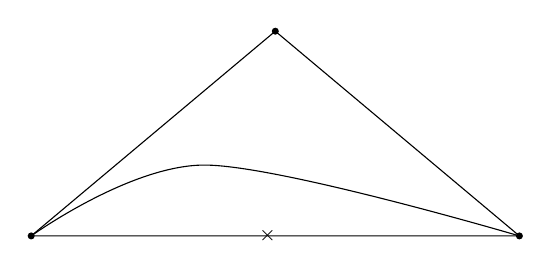
\begin{tikzpicture}[x=1mm,y=1mm,line cap=round,line join=round,font=\scriptsize]
\draw (18,-40) -- (49,-14) -- (80,-40) -- cycle;
\draw plot[smooth, tension=0.55] coordinates {(18,-40) (40,-31) (80,-40)};
\node[pt] at (18,-40) {};
\node[pt] at (49,-14) {};
\node[pt] at (80,-40) {};
\node[inner sep=1pt] at (48,-40) {\scriptsize $\times$};
\end{tikzpicture}
\end{document}
